\documentclass{svproc}

\usepackage{float}
\usepackage[T1]{fontenc}
\usepackage{url}
\usepackage{graphicx}
\usepackage{wrapfig}
\usepackage{listings}
\usepackage{color}

\renewcommand{\floatpagefraction}{.95}
\renewcommand{\topfraction}{.95}

\definecolor{blue}{rgb}{0.13,0.13,1}
\definecolor{green}{rgb}{0,0.5,0}
\definecolor{red}{rgb}{0.9,0,0}
\definecolor{grey}{rgb}{0.46,0.45,0.48}

\lstset{language=Java,
  commentstyle=\color{green},
  keywordstyle=\color{blue},
  stringstyle=\color{red},
  basicstyle=\ttfamily}

\lstdefinelanguage{ddlog}{
  language=Java, % we base it on Java, just for comments
  morekeywords={input, output, typedef, relation, typedef, bool,
    string, bit, extern, function, var, for, match, skip, in,
    Aggregate, FlatMap},
  deletestring=[b]{'}
}

\newcommand{\LR}[1]{\textbf{\color{red}LR: #1}}

\author{
        Leonid Ryzhyk \and
        Mihai Budiu}
\institute{VMware Research}

\title{Differential Datalog}

\date{}

\begin{document}
\maketitle

\section{Abstract}

%In distributed systems, the control plane is responsible for
%reconfiguring the system in response to external events.  Due to
%performance and scalability requirements, it is impractical to
%recompute the entire configuration on every update.  Instead,
%developers employ \emph{incremental algorithms} that update their
%outputs in response to input changes.  Such algorithms are notoriously
%hard to develop, leading to complex and inflexible implementations.
%(This is the classic ``incremental view update''
%problem~\cite{Gupta-sigmod93}).


Many real-world applications of deductive databases require
incrementally updating output tables in response to changes to input
tables.
To address this need, we have developed Differential Datalog
(DDlog), a dialect of Datalog that automates incremental computation.
A DDlog programmer only has to write a specification for the
original (non-incremental) problem.  Given this description, the DDlog
compiler generates an efficient incremental implementation.  The DDlog
runtime automatically maintains indexes required to efficiently
compute output updates.

The DDlog language is targeted for system builders.  In consequence,
the language emphasizes usability, by providing a rich type system,
a powerful expression language, including string manipulation, arithmetics,
and control flow constructs.  Finally, DDlog offers an
alternative syntax for writing Datalog rules, which has a more
imperative flavor.

\section{Introduction}\label{sec-introduction}

\subsection{Motivation}

Many real-world applications must update their output in response to input changes.  Consider, for
example, a cluster management system such as Kubernetes~\cite{kubernetes} that configures cluster
nodes to execute a user-defined workload.  As the workload changes, e.g., container instances are
added or removed from the system, the configuration must change accordingly.  In a large cluster,
computing configuration from scratch is prohibitively expensive.  Instead, modern cluster management
systems, including Kubernetes, apply changes incrementally, only updating state effected by the
change.

As another example, program analysis frameworks like Doop~\cite{Bravenboer-oopsla09} evaluate a set
of rules defined over the abstract syntax tree of the program.  Such an analyzer can be integrated
into the IDE to alert the developer as soon as a potential bug is introduced in the program.  This
requires re-evaluating the rules after every few keystrokes.  In order to achieve interactive
performance when working with very large code bases, the re-evaluation must occur incrementally,
preserving as much as possible intermediate results computed at earlier iterations.

Incremental algorithms tend to be significantly more complex than
their non-incremental versions.  In a nutshell, an incremental
algorithm propagates input changes to the output via all intermediate
steps.  This, in turn, requires (1) maintaining intermediate
computation results for each step, and (2) implementing an incremental
version of each operation, which, given an update to its input,
computes an update to its output.  Incremental computations that
operate on relational state are ubiquitous throughout systems
management software stacks.  The complexity of these algorithms
greatly impacts the development cost, feature velocity,
maintainability, and the performance of the control systems.

\emph{We argue that, instead of dealing with the complexity of
  incremental computation on a case-by-case basis,
  developers should embrace programming tools that solve the problem
  once and for all.}  In this paper we present one such tool -- \emph{Differential Datalog
  (DDlog)}~\cite{ddlog} -- a programming language that automates
incremental computation.  A DDlog programmer only has to write a
Datalog specification for the original (non-incremental) problem.  Given
this description, the DDlog compiler generates an efficient
incremental implementation.  

\subsection{Overview}

DDlog is a \emph{bottom-up}, \emph{incremental}, \emph{in-memory}, \emph{typed} Datalog engine for
writing \emph{embedded} deductive databases.

\textbf{Bottom-up:} DDlog starts from a set of ground facts (provided
by the user) and computes all possible derived facts by following
Datalog rules, in a bottom-up fashion.  (In contrast, top-down engines
are optimized to answer individual user queries without computing all
possible facts ahead of time.)  The bottom-up approach is preferable
in applications where all derived facts must be computed ahead of time
and in applications where the cost of initial computation is amortized
across a large number of queries.

\textbf{Incremental:} whenever the set of ground facts changes, DDlog
only performs the minimum computation necessary to compute all changes
in the derived facts.  This has significant performance benefits, and
only produces output of minimum size, minimizing communication
requirements.

\textbf{In-memory:} DDlog stores and processes data in
memory\footnote{In a typical use case, a DDlog program is used in
  conjunction with a persistent database; database records are fed to
  DDlog as inputs and the derived facts computed by DDlog are written
  back to the database; DDlog does not include a storage engine.}.  At
the moment, DDlog keeps all the data in the memory of a single
machine.  (This may change in the future, as DDlog builds on the
differential dataflow library~\cite{dd} that supports distributed
computation over partitioned data).

\textbf{Typed:} Pure Datalog does not have concepts like data types,
arithmetics, strings or functions.  To facilitate writing of safe,
clear, and concise code, DDlog extends Datalog with:
\begin{itemize}
\item A powerful type system, including Booleans, unlimited
  precision integers, bitvectors, strings, tuples, and
  Haskell-style tagged unions (but without recursive types).
  
\item The ability to store and manipulate sets, vectors, and maps as
  first-class values in relations, including performing aggregations.
  
\item Standard integer and bitvector arithmetic.
  
\item A simple procedural language that allows expressing many
  computations over these datatypes in DDlog without resorting to
  external functions.
  
\item String operations, including string concatenation and
  interpolation.
\end{itemize}

\textbf{Embedded:} while DDlog programs can be run interactively via a
command line interface, the primary use case is to run DDlog in the
same address space with an application that requires deductive
database functionality.  A DDlog program is compiled into a Rust
library that can be linked against a Rust, C/C++ or Java program
(bindings for other languages can be easily added).

DDlog is an open-source project, hosted on github~\cite{ddlog}, with a permissive MIT-license.

\section{Differential Datalog (DDlog)}\label{sec-ddlog}

A DDlog program operates on typed relations.  The programmer defines a
set of rules to compute a set of output relations based on input
relations (Figure~\ref{fig:differential}).  Rules are evaluated
incrementally: given a set of \emph{changes} to the input relations
(insertions or deletions), DDlog produces a set of changes to the
output relations (expressed also as insertions or deletions).

\begin{figure}[t]
    \center
    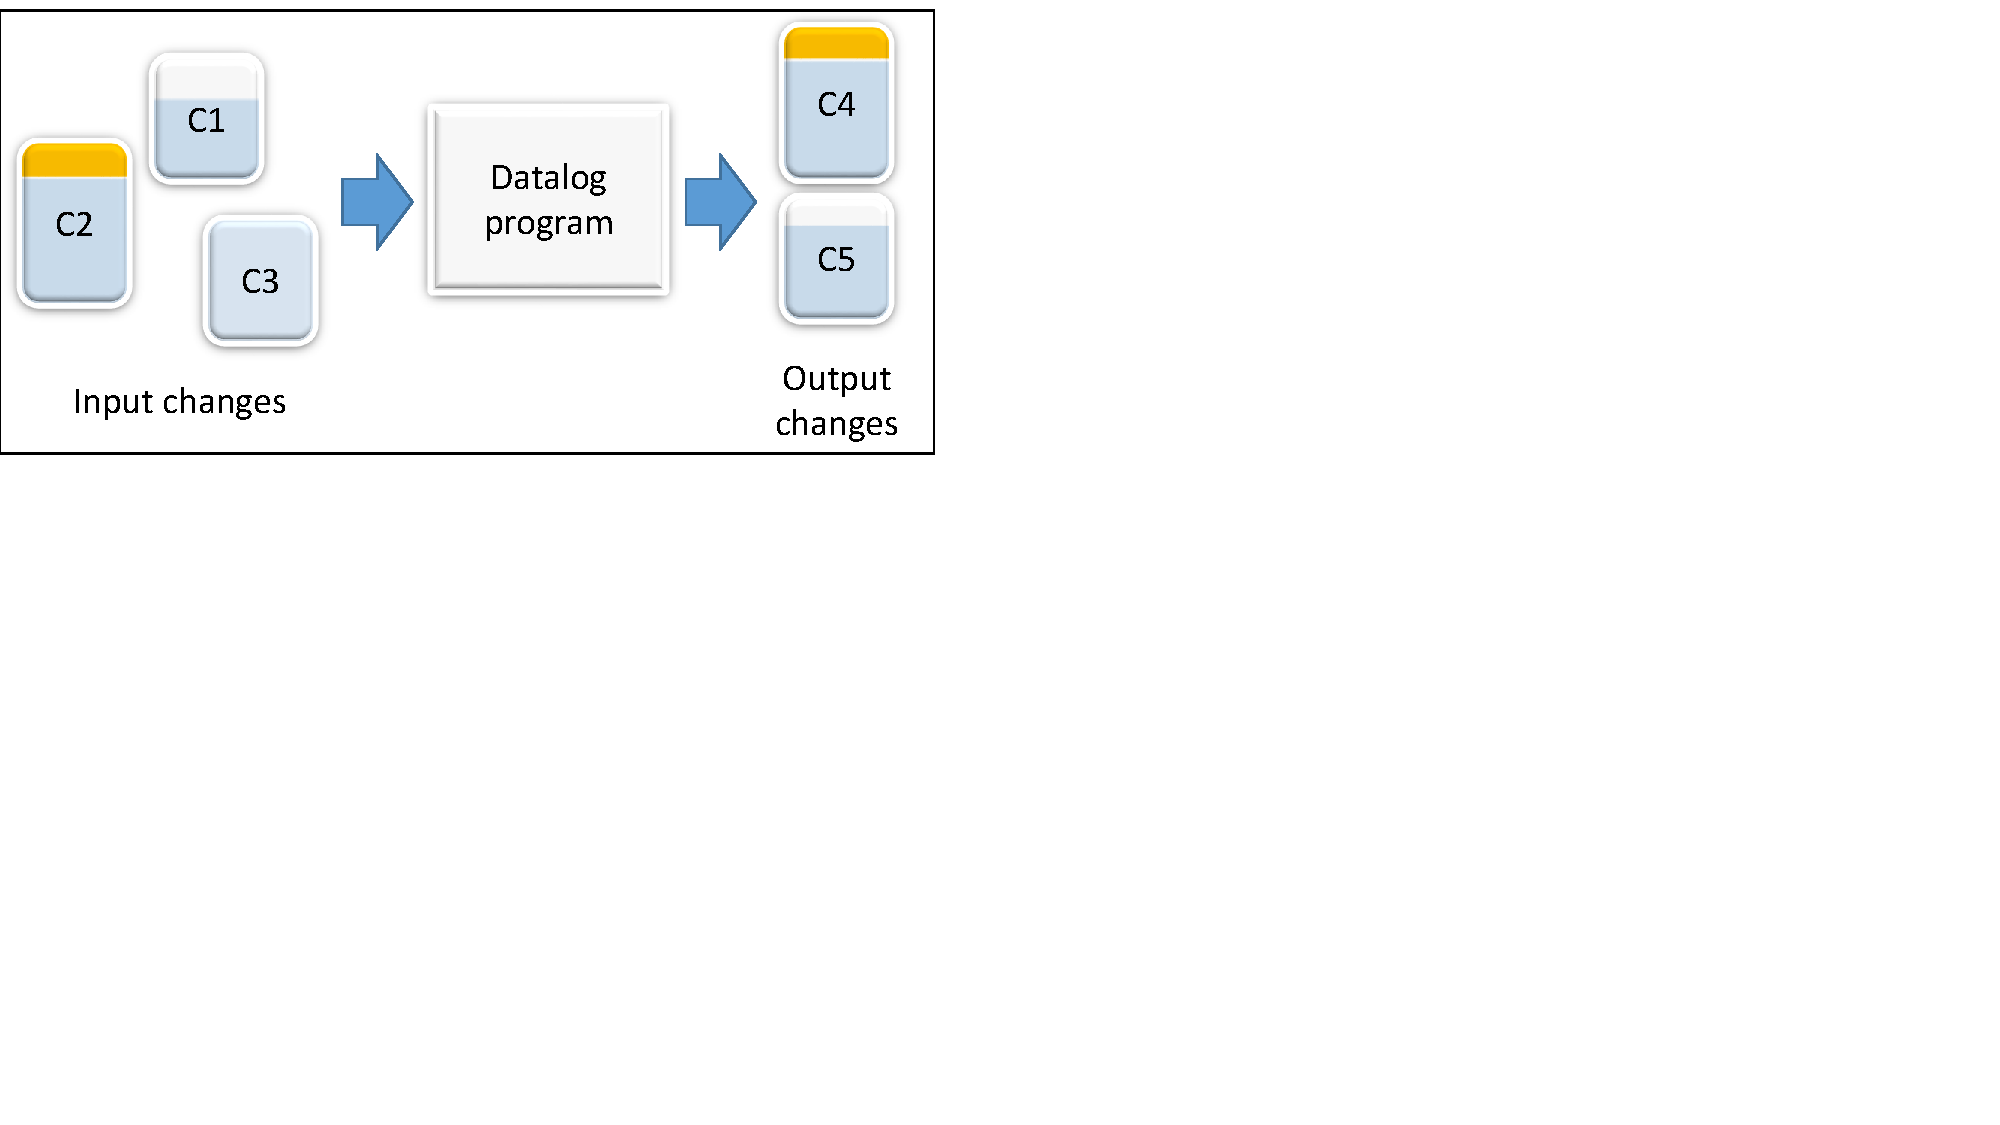
\includegraphics[width=0.5\columnwidth,clip=true,trim=0in 4.4in 6.5in 0in]{differential.pdf}
    \caption{Incremental evaluation of a Datalog program.\label{fig:differential}}
\end{figure}

Here we give a brief overview of the language; the DDlog language
reference~\cite{ddlog-manual} and tutorial~\cite{ddlog-tutorial}
provide a detailed presentation of language features.

\subsection{Type system.}

DDlog is a statically-checked, strongly-typed language; users specify
types for relations, variables, functions, but often DDlog can infer
types from the context.  The type system is inspired by Haskell, and
supports a rich set of types.  Base types include Booleans,
bit-strings (e.g., \texttt{bit<32>}), infinite-precision integers
(\texttt{bigint}), and UTF-8 strings.  Derived types are tuples,
structures, and tagged unions (which generalize enumerated types).  We
currently do not allow defining recursive types like lists or trees; however
DDlog contains three built-in collection types: maps, sets, and arrays
(described in Section~\ref{sec:collections}).  Figure~\ref{fig:types}
shows several type declarations.

Generic types are supported; type variables are syntactically
distinguished by a tick: \texttt{'A}.  The language
contains a built-in reference type \texttt{Ref<'T>}.  Unlike other
languages, two references are equal if the objects referred are equal;
thus references do not alter the nature of Datalog.  References can be
used to reduce memory consumption when complex objects are stored in
multiple relations.

\begin{figure}[t]
  \footnotesize
\begin{lstlisting}[language=ddlog]
// A tagged-union type
typedef IPAddress = IPv4Address{ipv4addr: bit<32>}
                  | IPv6Address{ipv6addr: bit<128>}
// A generic option type
typedef Option<'A> = None
                   | Some{value: 'A}
typedef OptionalIPAddress = Option<IPAddress>
\end{lstlisting}
\caption{Type declarations in DDlog.  \texttt{None}, \texttt{Some},
\texttt{IPv6Address} are \emph{pattern constructors}.\label{fig:types}}
\end{figure}

\subsection{Relations and Rules.}

Relations are strongly typed; the value in each column must have a
statically-determined type.  There are three kinds of relations in
DDlog:

\noindent \textbf{Input relations:} the content of these relations is provided by
the environment, in an incremental way.

\noindent \textbf{Output relations:} these are computed by the DDlog
program, and the DDlog runtime will inform the environment of changes
in these relations.

\noindent \textbf{Intermediate relations:} these are also computed by
the DDlog program, but they are hidden from the environment.

Figure~\ref{fig:relations-rules} shows three relation declarations.
An input relation may declare an optional primary key --- which is a
set of columns that can be used to delete entries efficiently by
specifying only the key.

\begin{figure}[t]
  \small
  \begin{lstlisting}[language=ddlog]
input relation Edge(from: node_t, to: node_t)
                    primary key (e) e.from
input relation Exclude(node: node_t)
output relation Path(src: node_t, dst: node_t)
/* The Path relation is computed as a union of two rules */
// Rule 1: base case
Path(x, y) :- Edge(x,y).
// Rule 2: recursive step: join Path relation with Edge
// followed by an antijoin with Exclude.
Path(x, z) :- Path(x, w), Edge(w, z), not Exclude(z).
  \end{lstlisting}
  \caption{A graph described by two relations and a rule to compute
    paths in the graph that exclude some nodes.\label{fig:relations-rules}}
\end{figure}

DDlog rules are composed of standard Datalog operators: joins, antijoins, and
unions, illustrated in Figure~\ref{fig:relations-rules}, as
well as aggregation, and flatmap, discussed in Section~\ref{sec:collections}.
DDlog allows recursive rules with stratified negation: intuitively, a DDlog
relation cannot recursively depend on its own negation.

\subsection{Computations in rules.}

Much of DDlog's power stems from its ability to perform complex
computation inside rules.  For example, the rule in
Figure~\ref{fig:area} computes an inner join of height and width
tables on the object id column, and then computes the area of the
object as the product of its height and width.

\begin{figure}[t]
  \footnotesize
  \begin{lstlisting}[language=ddlog]
input relation Height(object_id: int, height: int)
input relation Width(object_id: int, width: int)
output relation Area(object_id: int, area: int)
// Compute the area of an object as the product of
// its height and width.
Area(oid, area) :- Height(oid, h), Width(oid, w),
                   var area = w * h.

// Alternative syntax for defining the same relation.
for o in Height // o is a tuple with fields (object_id, height)
   for o1 in Width if o1.oid == o.oid
       Area(o.oid, o1.width * o.height)
  \end{lstlisting}
  \caption{Rule examples.  The first rule uses expressions and
    variables --- \texttt{var} introduces a \emph{variable binding}.
    The second rule is equivalent with the first one, but is written
    using an imperative-style syntax.\label{fig:area}}
\end{figure}

The DDlog expression language supports arithmetic, string
manipulation, control flow constructs and function calls.

\paragraph{Local variables.}
Local variables are used to store intermediate results of
computations.  In DDlog, local variables can be introduced in three
different contexts: (1) variables can be defined directly in the body
of a rule, e.g., the \texttt{area} variable in Figure~\ref{fig:area};
(2) a variable can be defined in a \texttt{match} pattern, as in
Figure~\ref{fig:function}; and (3) finally, a variable can be defined
inside an expression, e.g., the \texttt{res} variable in
Figure~\ref{fig:collections}.  A variable is visible within the
syntactic scope where it was defined.

\paragraph{``Imperative'' rule syntax.}
We have also defined an alternative syntax for rules, inspired by the
FLWOR syntax of XQuery expressions~\cite{boag-xquery02}.  The
``imperative'' fragment offers several statements: \texttt{skip} (does
nothing), \texttt{for}, \texttt{if}, \texttt{match}, block statements
(enclosed in braces), and variable definitions \texttt{var...in}.  An
example is shown in Figure~\ref{fig:area}.  This language is
essentially a language of monoid
comprehensions~\cite{fegaras-sigmod95}, so it is easily converted to a
traditional Datalog representation using a syntax-directed translation
in the compiler front-end.  Recursive relations cannot be expressed
using this syntax.

\paragraph{Integers.} The integer types (\texttt{bigint} and \texttt{bit<N>}) provide the
standard arithmetic operations, as well as bit-wise operations, bit
selection \texttt{v[15:8]}, shifting, and concatenation.

\paragraph{Strings} All primitive types contain built-in conversions to strings, and users
can implement string conversion functions for user-defined types (like
Java's \texttt{toString()} method).  Expressions enclosed within
\texttt{\$\{...\}} in a string literal are \emph{interpolated}: they
are evaluated at run-time, converted to strings and substituted; this
is a feature inspired by JavaScript; for example
\texttt{"x+y=\$\{x+y\}"}.

\begin{figure}[t]
  \footnotesize
  \begin{lstlisting}[language=ddlog]
function lastByte(a: OptionalIPAddress): bit<8> = {
  match (a) {
    None -> 0,
    Some{IPv4Address{.ipv4addr = addr}} -> addr[7:0],
    Some{IPv6Address{.ipv6addr = addr}} -> addr[7:0]
  }
}
relation Host(address: OptionalIPAddress)
// Rule that performs matching on address structure
IPv6Addr(addr) :- Host(.address=Some{IPv6Address{addr}}).
  \end{lstlisting}
\caption{Pattern matching used in a DDlog function and in a rule.\label{fig:function}}
\end{figure}

\paragraph{Pattern matching.}  DDlog borrows
the \texttt{match} expression from ML and Haskell; a \texttt{match}
expression simultaneously performs pattern-matching against type
constructors or values, and also can bind values.
Figure~\ref{fig:function} shows a \texttt{match} expression that uses
a nested pattern to extract a byte from a value \texttt{a} with type
\texttt{OptionalIPAddress} (this type was defined in
Figure~\ref{fig:types}).  For example, the last case binds the
\texttt{addr} variable to the value of the \texttt{ipv6addr} field.

Pattern matching can also be used directly in the body of a rule, as
in the last line from Figure~\ref{fig:function}, which extracts only
IPv6 addresses from the \texttt{Host} relation and binds their value
to the \texttt{addr} variable, which in turn is used in the left-hand side of
the rule defining \texttt{IPv6Addr} relation.

\paragraph{Functions.}

DDlog functions encapsulate pure (side-effect-free) computations.
Example functions are \texttt{lastByte} from
Figure~\ref{fig:function}, and \texttt{concat} from
Figure~\ref{fig:collections}.  Recursive functions are not supported.
Users and libraries can declare prototypes of \texttt{extern}
functions, which must be implemented outside of DDlog (e.g., in Rust),
and linked against the DDlog program at link time.  The compiler
assumes that extern functions are pure.

\subsection{Collections}\label{sec:collections}

The DDlog standard library contains three built-in generic collection
types (implemented natively in Rust): \texttt{Vec<'T>},
\texttt{Set<'T>} and \texttt{Map<'K, 'V>}.  Values of these types can
be stored as first-class values within relations.  Equality for values
of these types is defined element-wise.  In theory such types are not
necessary, since collections within relations can be represented using
separate relations.  We have introduced them into the language because
many practical applications have data models that contain nested
collections; by supporting collection-valued columns natively in DDlog
we can more easily interface with such applications, without the need
to write glue code to convert collections back and forth into separate
relations using foreign keys.

Figure~\ref{fig:collections} shows the declaration in DDlog of an
external function which splits a string into substrings using a
separator; this function returns a vector of strings.

\begin{figure}[t]
  \footnotesize
  \begin{lstlisting}[language=ddlog]
// declare external function returning a vector of strings
extern function split(s: string, sep: string): Vec<string>
// DDlog function to concatenate all elements of a vector
function concat(s: Vec<string>, sep: string): string = {
  var res = "";
  for (e in s) {
    res = (if (res != "") (res + sep) else res) + e
  };
  res   // last value is function evaluation result
}

input relation Phrases(p: string)
relation Words(w: string)
// Words contains all words that appear in some phrase
Words(w) :- Phrases(p), var w = FlatMap(split(p, " ")).

// Shortest path between each pair of points x, y
// (x, y) is the key for grouping
// min is the function used to aggregate data in each group
ShortestPath(x, y, min_cost) :- Path(x, y, cost),
                 var min_cost = Aggregate((x, y), min(cost)).
\end{lstlisting}
\caption{Operations on collections: iteration, flattening,
  aggregation.\label{fig:collections}}
\end{figure}

\texttt{for} loops can be used to iterate over elements in
collections.  Figure~\ref{fig:collections} shows an implementation of
the function \texttt{concat}, the inverse of \texttt{split}, which
uses a loop.

The \texttt{FlatMap} operator can be used to flatten
a collection into a set of DDlog records, as illustrated in the definition of
relation \texttt{Words} in Figure~\ref{fig:collections}.

The \texttt{Aggregate} operator can be used to evaluate the equivalent
of SQL groupby-aggregate queries.  The aggregate operator has two
arguments: a key function, and an aggregation function.  The
aggregation function receives a group of
records that share the same key.  The
\texttt{ShortestPath} relation in Figure~\ref{fig:collections} is
computed using aggregation.

\subsection{Module system}

DDlog offers a simple module system, inspired by Haskell and Python,
which allows importing definitions (types, functions, relations) from
multiple files.  The user can add imported definitions directly into the
name space of the importing module or keep them in a separate name space to
prevent name collisions.  Similar to Java packages, module names are
hierarchical and the module name hierarchy must match the paths on the
the filesystem where modules are stored.  The directive \texttt{import
  library.module} will load the module from file
\texttt{library/module.dl}.

The DDlog \emph{standard library} is a module containing a growing
collection of useful functions and data structures: some generic
functions and data-types, such as \texttt{min}, string manipulation
and conversion to strings, functions to manipulate vectors, sets, maps
(insertion, deletion, lookup, etc.).

%\subsection{``Imperative'' relation definitions}

\section{DDlog Implementation}\label{sec-system}

\subsection{Compiling DDlog to Differential Dataflow}

Figure~\ref{fig:compiler-flow} shows how DDlog programs are compiled
into native code.  The DDlog compiler is written in Haskell.  The
compiler performs parsing, type inference, validation, and several
optimization steps; it generates Rust code (as text files); the Rust
code is compiled and linked with the Differential Dataflow (DD)
library~\cite{differential-dataflow} to produce a static or dynamic
native code library.  DD is an independent open-source
project~\cite{differential-dataflow}, described in a series of
publications~\cite{timely-dataflow,differential-dataflow-paper} and
online documents~\cite{dd-mdbook,dd-reference}.  DD can be executed
using multiple cores or even multiple shared-nothing machines, but we
currently only support a single machine.

The output of the DDlog compiler, and the input to the DD library is a
dataflow graph, which may contain cycles (cycles are introduced by
recursion).  The edges of the dataflow graph are typed relations, and
the nodes are dataflow relational operators.  DD natively implements
the following operators: join, antijoin, distinct, union, aggregation,
filter, and flatmap.  Each operator has a highly optimized
implementation, incorporating temporal indexes that keep multiple
versions of each relation and allow efficient incremental evaluation.
The DD runtime library is responsible for executing the emitted
dataflow graph across many cores, in a transactional fashion.  The
DD runtime can be allocated a specific number of threads.

\subsection{Transactional API}

The interaction with a running DDlog program is done through a
transactional API.  At any time only one transaction can be
outstanding.  After \texttt{start}ing a transaction the users can
insert and delete any number of tuples from input relations.  When
attempting to \texttt{commit} a transaction all updates are applied
atomically and changes to all output relations are produced.  Users
can register an upcall to be notified of these changes.  These
notifications will happen on different threads, while the thread
executing the \texttt{commit} is blocked.  Figure~\ref{fig:javaapi}
shows an example Java program that interacts with a DDlog program.

\subsection{The command-line interface}

For every DDlog program the compiler generates an executable library,
a Rust program that allows invoking the DDlog program from Rust, and a
command-line interface program (CLI) that allows users to interact
with the DDlog program directly.  The CLI allows users to start
transactions, insert or delete tuples in input relations, commit
transactions, dump the contents of relations, and get statistics
about resource consumption.  The CLI is used for regression testing
and debugging.

\subsection{C and Java interfaces}

The compiled DDlog program exposes a transactional API to add and
delete records from input relations and notify the application about
changes in output relations at runtime.  The API is natively
implemented in Rust, with bindings available for other languages,
currently C and Java.  The Java API is program-independent, but the
native executable needs to be regenerated every time the DDlog program
is changed.  We illustrate the Java API to a simple DDlog with a
skeleton example in Figure~\ref{fig:javaapi}.

\begin{figure}[t]
  \footnotesize
  \begin{lstlisting}[language=ddlog]
// DDlog program    
input relation Parent(parent: string, child: string)
output relation Ancestor(ancestor: string, descendant: string)
Ancestor(ancestor, descendant) :- Parent(ancestor, descendant).
Ancestor(ancestor, descendant) :- Ancestor(ancestor0, ancestor1),
                                  Parent(ancestor1, descendant).
  \end{lstlisting}
  
  \begin{lstlisting}[language=Java]
// Java program interfacing with DDlog program    
static class Parent {
  String parent;
  String child; }
static class Ancestor {
  String ancestor;
  String descendant; }

/* Instantiate the DDlog program; add a record to the
 * Parent relation. */
static void main() {
  DDlogAPI api = new DDlogAPI(2 /* threads */,
               r -> onCommit(r) /* callback */);
  int parentRelation = api.getTable("Parent");
  Parent p = new Parent();
  p.parent = "Mike"; p.child  = "John";
  /* Create DDlog insert command. */
  DDlogCommand command = new DDlogCommand(
     DDlogCommand.Kind.Insert, parentRelation, p);
  int exitcode = api.start();  // start transaction
  DDlogCommand[] commands = new DDlogCommands[1];
  commands[0] = command;
  exitcode = api.applyUpdates(commands);
  /* commit transaction; causes the callback to be 
   * invoked for each new or deleted output record.
   * commit blocks until all upcalls have been invoked. */
  exitcode = api.commit();
  api.stop();
}

/* Callback invoked on commit once for each insertion or
 * deletion in an output relation. */
static void onCommit(DDlogCommand command) {
  int outputRelation = command.tableId;
  Ancestor value = command.getObject<Ancestor>();
  if (command.kind == DDlogCommand.Kind.Insert) 
    // ancestor inserted
  else 
    // ancestor deleted
}
\end{lstlisting}
\caption{Example program showing the Java API to pass and receive data
  from a DDlog program.\label{fig:javaapi}}
\end{figure}

\section{Applications}\label{sec:applications}

\subsection{Controller for Virtual Networks}

The most significant DDlog program we have written so far is a
reimplementation of OVN~\cite{ovn} -- a production-grade
virtual network controller used to implement the network substrate
for cloud management systems.

OVN translates a set of network management policies into OpenFlow
rules that have to be installed on the virtual switches in the
network.  The logic is very complicated, comprising tens of input,
output and intermediate relations.

The original program was written in C, and is not fully incremental.
The DDlog implementation has about 6000 lines of code, about the same
size as the original code base, but it is fully incremental.
With the exception of a small number of library functions imported
from C, we were able to implement the entire OVN logic in DDlog.
This would not be feasible with a more traditional dialect of Datalog
that does not support types and expressions, as we relied on these
features extensively in our implementation.

%The original
%program builds an in-memory object model of the database; in that
%implementation joins with a primary key become just pointer
%dereferences.  Moreover, some operations are implemented using
%side-effects and are challenging to do in a declarative model; an
%example is allocation of network addresses, where new addresses are
%allocated using a counter, to prevent old addresses from being reused
%for as long as possible.  The original program generates open-flow
%rules encoded as strings, so this implementation makes extensive use
%of the string interpolation facilities of DDlog.

Preliminary evaluation indicates that the incremental performance is
several orders of magnitude better than the original program for large
networks.  Figure~\ref{fig:ovn_perf} compares the cost of applying a small incremental
change to network reconfiguration for varying network sizes for
C and DDlog versions of the program.

\begin{figure}
    \center
    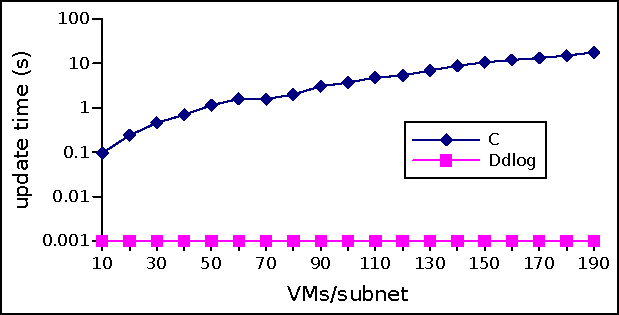
\includegraphics[width=0.4\columnwidth]{update_plot.pdf}
    \caption{The cost of incremental network updates.\label{fig:ovn_perf}}
\end{figure}

%TODO: how well does it work.

\subsection{Program analysis}

We have evaluated DDlog on a large Datalog program written for the
Souffle Datalog compiler.  The Datalog program performs many
compiler analyses simultaneously, computing their fixed-point.  We
have written a Python program that converts a large subset of the
Souffle Datalog syntax into DDlog (we have manually handled the
missing features).  The input program consists of 580 lines, and the
input dataset consists of 3.5 million tuples.

The non-incremental Souffle Datalog engine used by Doop evaluates the
program on this dataset in 23 seconds, whereas DDlog takes 45 seconds.
After the initial evaluation, DDlog propagates small updates, adding or
removing several input records, in under 10ms.  

A hand-optimized version of the program, provided by Doop developers,
reduces the evaluation time to 1 second by using the join order
optimization.  DDlog does not currently allow the developer to
control join evaluation order, which prevents us from reproducing the
same optimization.

%TODO: how well does it work?

%\subsection{Firewall management}
%
%We have reimplemented a proprietary network management application in
%DDlog.  The application manages a firewall in a network of switches
%and virtual machines (VMs).  The firewall is driven by a centralized
%policy.  The centralized policy is implemented in a distributed
%fashion by the VMs and network switches, each of which performs
%filtering using local rules.  When the centralized policy changes, the
%local rules have to be updated in all network devices.  The core
%of this program is a graph reachability problem, which is written in a
%few lines of DDlog.  The DDlog program outperformed a hand-optimized
%Java implementation consisting of several thousand lines of code
%by a factor of 3 to 8.

\section{Related work}

There is significant work building Datalog engines for various
purposes: Souffle~\cite{scholz-cc16} (program analysis),
Doop~\cite{Bravenboer-oopsla09} (program analysis),
LogiQL~\cite{Borraz-Sanchez-dlp18} (integer linear programming),
Vadalog~\cite{Bellomarini-vldb18} (existential quantification),
DeALS~\cite{Yang-vldb17} (concurrent execution),
DataFun~\cite{Arntzenius-icfp16} (higher-order functional
programming), NDLog~\cite{loo-cacm09} (declarative networking),
SociaLite~\cite{Seo-vldb13} (large scale graph analysis),
and~\cite{Barany-tods17} (probabilistic programming).  A survey can be
found in~\cite{Maier-book18}.

The only other incremental Datalog engine that we are aware of is a
LogiQL~\cite{Green-pods15}, a commercial product of
LogicBlox~\cite{Aref-sigmod15}.

DDlog is built on top of Differential Dataflow~\cite{dd}; several
interesting declarative query engines were built on top of
DD~\cite{timely-dataflow,differential-dataflow-paper}.

Some of the DDlog features were inspired by .Net
LINQ~\cite{meijer-dpcool03,Meijer-sigmod06}.

There is also significant work on incremental computation systems;
some of these are for much richer computation
models~\cite{acar-05,Carlsson-icfp02,Demetrescu-oopsla11,harkes-ecoop16,Hammer-pldi14},
and some just for relational
models:~\cite{ahmad-vldb12,Szabo-ase016,zhao-icmd17}.

\section{Conclusion and future work}\label{sec-conclusions}

DDlog is a young project.  The language is evolving quickly, driven by
the use cases.  We place paramount importance on language usability;
this is why we have enhanced Datalog with many non-traditional
constructs.  Our goal is to reduce as much as possible the need to
transition between multiple languages when writing large projects.

TODO


\bibliographystyle{abbrv}
\bibliography{top}

\end{document}
